\section{Decision criteria}
\label{sec:decision}

A common observation is that increasing the grid resolution or the polynomial degree of the basis functions will decrease the difference between the finite element approximation $u_\text{hp}$ and the actual solution $u$.

In fact, the impact of these adaptation techniques on this error is well understood. \textcite[Thm.~3.4]{babuska1990} determined an upper bound for the error that depends both on the cell diameter $h$ and the polynomial degree $p$:
\begin{align}
\label{eq:errorbound_hp} \left\|e_\text{hp}\right\|_{H^{1}(\Omega)} &\leq C \, h^{\mu} \, p^{-(m-1)} \, \|u\|_{H^{m}(\Omega)} \,\text{,}
\end{align}
where $e_{hp} = u - u_\text{hp}$ denotes the error function, $m$ is a measure for the regularity of the solution $u$, $C$ is a constant dependent on $m$, and $\mu = \min \left(p, m - 1\right)$.

These modifications do not have to happen uniformly on a global scale, but can be applied locally, since the global error consists of the local ones of each cell $K$:
\begin{align}
\label{eq:error_sum} \left\|e_\text{hp}\right\|_{H^1(\Omega)}^2 = \sum\limits_{K \in \Omega} \left\|e_\text{hp}\right\|_{H^1(K)}^2 \,\text{.}
\end{align}
Thus it all comes down to find those sections that have a significant contribution to the global error, and mitigate their impact by local adaptation. \textcite[Thm.~5.1]{guo1986} predicted exponential convergence with the number of \glspl{dof} $n_\text{dofs}$ on a suitable \hp-adapted mesh:
\begin{align}
\label{eq:errorbound_exp} \left\|e_\text{hp}\right\|_{H^{1}(\Omega)} &\leq C \, \exp\left(- b \, n_\text{dofs}^{1 / 3}\right) \,\text{,}
\end{align}
where constants $b > 0$ and $C$ are both independent of $n_\text{dofs}$.

With sufficient information about the investigated scenario, an \hp-adaptive grid can be tailored to its specifics manually. However, grid adjustments by hand may not be optimal. Furthermore, not all peculiarities about the scenario are generally known in advance, which is especially the case for problems with complex geometries and time dependent ones.

Hence we need to elaborate on algorithms to automatically decide which subsets of the domain qualify for adaptation. With this technique, we typically set up a coarse mesh along with basis functions of a low polynomial degree and obtain a tailored mesh after several adaptation iterations.

In this section, we present different ways to identify areas whose adaptation will be most profitable, and to choose the most beneficial type of adaptation. For hp-adaptation in particular, \textcite{mitchell2014} reviewed and compared a selection of strategies in detail. We demonstrate a subset of their recommendations in terms of performance and applicability, i.e.\@ those strategies that only require locally relevant part of the current solution.



\subsection{Adaptation strategies}
\label{ssec:strategy}

We will decide on the basis of adaptation criteria for every cell which ones will be considered to be adapted. Typical criteria involve comparing errors or their estimates to some absolute or relative threshold. Alternatively, also predicted errors or smoothness indicators are used for this purpose, as presented in the following sections. \textcite[Sec.~5.2]{bangerth2003} describe non-trivial strategies on how to decide based on these adaptation criteria, from which we present a commonly used selection.

So called \textit{fixed-error-reduction} or \textit{fixed-fraction} strategies select subsets of cells whose criteria accumulate to a predefined fraction of their global sum. This strategy is only applicable when the sum of all criteria actually has meaning, for example local errors which add up to the global one. Further, it may lead to optimal meshes for several problems, but tends to only adapt very few cells whenever singularities are encountered. We will use this strategy in our applications presented in Ch.~\ref{ch:results}.

On the other hand, strategies known as \textit{fixed-rate} or \textit{fixed-number} pick predefined fractions of cells with the lowest or highest criteria for adaptation. This allows to predict the growth of cells, but may not lead to an optimal mesh since more cells may be adapted than necessary.

For either strategy, when using actual errors or error indicators as adaptation criteria, we typically select the subset of cells corresponding to the higher error for refinement, while the subset with the lower error is considered for coarsening.

Applicable implementations of these strategies involve binary searches to determine the section of cells relevant for adaptation. For parallel computations, according algorithms have been developed by \textcites[Sec.~3.1]{burstedde2008}[Sec.~5.1]{bangerth2012}.



\subsection{Error estimation}
\label{ssec:estimation}

The determination of the error for our finite element approximation requires the actual solution to be at our disposal. However, this is not the case in general, and we need to come up with an alternative measure.

\textcite{kelly1983} worked out an \textit{a posteriori} error estimator for the generalized Poisson equation $-\nabla \cdot \left( a \nabla u \right) = f$, where $a$ is a function usually describing material characteristics. They determined an upper bound $\eta_K$ for the error on each cell by balancing the gradient of the finite element approximation $u_\text{hp}$ on all faces $F$ of the cell's boundary:
\begin{align}
\label{eq:kelly} \|e_\text{hp}\|_{H_1(\Omega)}^2 &\leq C \sum\limits_{K \in \Omega} \eta_K^2 &&\text{with}&  \eta_K^2 &= \sum\limits_{F \in \partial K} c_F \int\limits_{F} \left[ a \, \frac{\partial u_\text{hp}}{\partial n} \right]^2 \differential{o} \,\text{,}
\end{align}
where $C$ is independent of the solution, but depends on $a$, and
\begin{align*}
\left[ a \, \frac{\partial u_\text{hp}}{\partial n} \right] = \left. a \, \frac{\partial u_\text{hp}}{\partial n_K} \right|_K + \left. a \, \frac{\partial u_\text{hp}}{\partial n_J}\right|_J
\end{align*}
denotes the jump of the approximation's gradient on the face between two adjacent cells $K$ and $J$. Hence \textcite{ainsworth1997a} attribute this estimator to the class of gradient recovery estimators.

The constant $c_F$ depends on the characteristics of each individual face of the cell. \textcite{kelly1983} originally used the constant $c_F = \frac{h_K}{24 \, a_\text{min} \, p_K}$ on each face, on which we determine the minimum $a_\text{min}$ of the given function. Here, $h_K$ and $p_K$ denote both cell diameter and polynomial degree of the finite element on cell $K$, respectively. \textcite{davydov2017} proposed a different constant for \hp-adaptive \gls{fem}: They recommend $c_F = \frac{h_F}{2 \, a_\text{min} \, p_F}$ with $h_F$ the face diagonal and $p_F = \max\left(p_K, p_J\right)$ the largest polynomial degree of adjacent elements $K$ and $J$ on this particular face.

This estimator has been worked out for the Poisson equation, but has proven its applicability on other problems as well, where this is no longer meant to be an estimator, but rather an error indicator \cite{dealiikelly}.

The error estimator is already implemented in \dealii{} \cite{dealiikelly}.

We will use these error estimates to decide w. We are still left to decide which type of adaptation we want to apply, i.e.\@ \h-adaptation or \p-adaptation.



\subsection{Error prediction}
\label{ssec:prediction}

\cite{babuska1990} determined upper error bounds for numerical solutions based the distribution of finite elements. Both mesh resolution and polynomial degrees of the basis functions have a different, yet quantifiable influence on the error leading to Eq.~(\ref{eq:errorbound_hp}).

Their findings are valid not only for the numerical solution on a global scope, but on subsets of the domain as well. Local changes by \h- and \p-adaptation will thus result in different local error bounds. This motivates a strategy to locally decide which type of adaptation to impose based on the refinement history which has been proposed by \textcite{melenk2001}: We can predict how the current error will change whenever certain areas of our domain are considered for adaptation in the following iteration. These predicted error estimates allow us to decide whether the choice of adaptation in the previous step was justified, and provide the foundation for it on the next one.

We determine how the error bounds on two different distributions of finite elements will change by calculating their ratio. For this, we assume that both the actual error and its upper bound change with the same rate, which allows us to equate both ratios. We further assume that the solution is sufficiently regular ($m \gg p$). The ratio of errors then reads:
\begin{align}
\label{eq:errorratio_hp} \frac{\left\|e_{h_\text{f} p_\text{f}}\right\|_{H^{1}(\Omega)}}{\left\|e_{h_\text{a} p_\text{a}}\right\|_{H^{1}(\Omega)}} = \frac{h_\text{f}^{p_\text{f}}}{h_\text{a}^{p_\text{a}}} \, \left(\frac{p_\text{f}}{p_\text{a}}\right)^{-(m-1)} \,\text{,}
\end{align}
where subscripts $a$ and $f$ denote the finite element that is currently active or will be active after adaptation, respectively.

If we only consider \h-adaptation and leave the polynomial degree of the basis function unchanged ($p_\text{f} = p_\text{a} \equiv p$), we end up with the classical error bound \todo{cite}:
\begin{align}
\label{eq:errorratio_h} \frac{\left\|e_{h_\text{f} p}\right\|_{H^{1}(\Omega)}}{\left\|e_{h_\text{a} p}\right\|_{H^{1}(\Omega)}} = \left( \frac{h_\text{f}}{h_\text{a}} \right)^p \,\text{.}
\end{align}

However, if only \p-adaptation is considered and we keep the domain unchanged ($h_\text{f} = h_\text{a} \equiv h$), the ratio of errors still depends on the regularity of the actual solution which is not at our disposal in general. Following the considerations of \cite{melenk2001}, we expect \p-adaptation to change the error exponentially with the increment of the polynomial degree:
\begin{align}
\label{eq:errorratio_p} \frac{\left\|e_{h p_\text{f}}\right\|_{H^{1}(\Omega)}}{\left\|e_{h p_\text{a}}\right\|_{H^{1}(\Omega)}} = h^{p_\text{f} - p_\text{a}} \, \left(\frac{p_\text{f}}{p_\text{a}}\right)^{-(m-1)} \simeq c^{p_\text{f} - p_\text{a}} \,\text{,}
\end{align}
where $c$ is a constant independent of the cell diameter $h$.

We suggest a similar approach for the \hp-adaptation case as well. The above ratio assumes that the underlying mesh has not been changed. We thus identify Eq.~(\ref{eq:errorratio_p}) with an unaltered cell diameter ($h \equiv h_\text{a}$) in Eq.~(\ref{eq:errorratio_hp}) resulting in:
\begin{align}
\label{eq:errorratio_hp_exp} \frac{\left\|e_{h_\text{f} p_\text{f}}\right\|_{H^{1}(\Omega)}}{\left\|e_{h_\text{a} p_\text{a}}\right\|_{H^{1}(\Omega)}} \simeq \left( \frac{h_\text{f}}{h_\text{a}} \right)^{p_\text{f}} \, c^{p_\text{f} - p_\text{a}} \,\text{.}
\end{align}

Now, we will use these findings to develop an algorithm to predict errors of our finite element approximation. \textcite{melenk2001} worked out such an algorithm for \hp-refinement, which we will extend to \hp-coarsening as well. First, we will now only consider individual cells on our domain rather than the whole domain itself. Further, in practical applications, the actual error on these may be not at our disposal. Instead, we use suitable error indicators $\left\|e_{hp}\right\|_{H^{1}(K)} \simeq \eta_K$, assuming that they change with the same rate as the actual error.

We apply our consideration summarized in Eq.~(\ref{eq:errorratio_hp_exp}) on any form of adaptation. However, \h-adaptation poses an additional challenge, since we have to distribute errors from parent to children cells in case of refinement, or combine them in reverse for coarsening. Here, we will only consider isotropic \h-adaptation of quadrilaterals in two and hexahedrals in three dimensions, so that exactly $2^\text{dim}$ children are assigned to a cell, and the ratio of cell diameters $h_\text{f} / h_\text{a}$ is fixed to be $0.5$ for refinement and $2$ for coarsening. Further, the predicted error of a refined cell is distributed equally on all of its children, while the error of all coarsened cells is summed up for their parent. We assign future finite elements with their corresponding polynomial degrees on parent and children cells as described in Sec.~\todo{add reference}. Last, like to \textcite{melenk2001}, we introduce control parameters $\gamma_n, \gamma_h \in (0, \infty)$, as well as $\gamma_p \in (0,1)$ for all three forms of adaptation, i.e.\@ no, \h-, and \p-adaptation. We end up with a set of equations which covers all possible combinations for \hp-adaptation:
\begin{align}
&\text{no adaptation:} & \eta^\text{pred}_K &= \eta_K \, \gamma_n \,\text{,} \\
&\text{\p-adaptation:} & \eta^\text{pred}_K &= \eta_K \, \gamma_p^{p_{\text{f},K} - p_{\text{a},K}} \,\text{,} \\
&\text{\hp-refinement:} &\eta^\text{pred}_{K_c} &= 0.5^{\text{dim}} \, \eta_{K_p} \, \gamma_h \, 0.5^{p_{\text{f},K_c}} \, \gamma_p^{p_{\text{f},K_c} - p_{\text{a},K_p}} \,\text{,} \\
&\text{\hp-coarsening:} & \eta^\text{pred}_{K_p} &= \sum\limits_{c} \eta_{K_c} \left( \gamma_h \, 0.5^{p_{\text{f},K_p}} \right)^{-1} \, \gamma_p^{p_{\text{f},K_p} - p_{\text{a},K_c}} \,\text{.} 
\end{align}
To clarify roles during \h-refinement and \h-coarsening, we marked parent cells $K_p$ and their children $K_c$ with corresponding subscripts, respectively.

We now have an algorithm to predict the error for the next adaptation step on basis of the current one. We are left to find a suitable criterion on how to use it to actually decide .

The original idea of \cite{melenk2001} was to compare the actual error of a cell $\eta_K$ in an adaptation cycle to its prediction $\eta_K^\text{pred}$ from the previous cycle. On all cells flagged for refinement, they consider \h-refinement for $\eta_K > \eta_K^\text{pred}$ and \p-refinement otherwise. We will extend these consideration to work for coarsening as well: For this, we need to pick the according strategy that keeps the cell diameter $h_k$ small for $\eta_K > \eta_K^\text{pred}$, and the polynomial degree $p_K$ large otherwise. The motivation behind this particular choice is that we keep the grid resolution fine whenever we suspect a singularity, which is usually indicated by a local error larger than its prediction.

An alternative approach would be to use the \textit{fixed-fraction} adaptation strategy from above: As indicators for each cell, we calculate the difference of predicted and estimated errors $(\eta_K^\text{pred} - \eta_K)$ for each subset of cells flagged for refinement and coarsening, respectively. On cells to be refined, we consider the fraction corresponding to the largest values for \p-adaptation, while for cells to be coarsened, the fraction with the lowest values will be picked. This conforms to the same argumentation as in the original variant. We will use this strategy in our applications presented in Ch.~\ref{ch:results}.

In practice, we need all predicted errors already for the initialization of this method. We provide them with an initial \h- or \p-adaptation of the mesh, by setting all predicted errors to $\eta_K^\text{pred} = 0$ or $\eta_K^\text{pred} = \infty$, respectively. We recommend to begin with an initial \h-refinement since its error predictor from Eq.~(\ref{eq:errorratio_h}) tends to be more reliable.

The error predictor has been implemented in the \dealii{} library as part of this dissertation. A development log can be found here \textcite{dealiipr8341}.



\subsection{Smoothness estimation}
\label{ssec:smoothness}

According to Eq.~(\ref{eq:errorbound_hp}), we notice that \p-adaptation has the largest impact on the error if its corresponding solution is sufficiently regular. Thus, determining the smoothness of the finite element approximation presents a reasonable indicator to decide between \h- and \p-adaptation.

The basic idea to quantify smoothness involves the transformation of the finite element approximation into its spectral representation. In one dimension, we expand it into a series of $L_2$-orthogonal basis functions $(P_k)_{k\in\mathbb{N}_0}$ on an interval $I = [a,b]$ with:
\begin{align}
u_{hp}(x) &= \sum\limits_{k \geq 0} c_k P_k(x) \,\text{,} && \forall x \in I \,\text{,} \\
\langle P_k, P_l \rangle &= 0 \,\text{,} && \forall k,l \in \mathbb{N}_0 \text{,}~ k \neq l \,\text{,}
\end{align}
and identify the smoothness as the rate of decay of the expansion coefficients $c_n$. In multi-dimensional cases, we formulate the expansion in the multi-index notation with tuples $\mathbf{k} = (k_1, \dots, k_\text{dim}) \in N_0^\text{dim}$ on each cell $K$:
\begin{align}
u_{hp}(\vec{x}) &= \sum\limits_{k_1 \geq 0} \dots \sum\limits_{k_\text{dim} \geq 0} c_{k_1, \dots, k_{\text{dim}}} P_{k_1, \dots, k_{\text{dim}}}(\vec{x}) = \sum_{\mathbf{k} \geq 0} c_\mathbf{k} P_\mathbf{k}(\vec{x}) \,\text{,}  & \forall \vec{x} \in K \,\text{,}
\end{align}
where we consider the multi-dimensional expansion as a product of basis functions for every coordinate direction:
\begin{align}
\label{eq:spectral_multi} P_{\mathbf{k}}(\vec{x}) &\coloneqq P_{k_1}(x_1) \dots P_{k_\text{dim}}(x_\text{dim}) \,\text{.}
\end{align}

In the following, we will present two different ways to estimate its smoothness with this method, namely with Legendre and Fourier series expansions.

\textcite{mavriplis1994} were the first to attribute smoothness characteristics to the decay of coefficients from a Legendre series expansion. Legendre polynomials are solutions to the Legendre differential equation on the interval $I=[-1,1]$:
\begin{align}
\frac{d}{d x}\left(\left(1-x^{2}\right) \frac{d}{d x} P_{n}(x)\right)+ n \left(n+1\right) P_{n}(x)=0 \,\text{.}
\end{align}
They can be constructed with Rodrigues formula and fulfill the orthogonality criterion
\begin{align}
P_j(x) &= \frac{1}{2^j j!} \frac{\text{d}^n}{\text{d}x^n} \left( \left(x^2 - 1\right)^n \right) \,\text{,} \\
\label{eq:legendre_orthogonal} \langle P_{m}, P_{n}\rangle &= \frac{2}{2 n+1} \delta_{m n} \,\text{.}
\end{align}
The first few polynomials are depicted in Fig.~\ref{fig:legendre}. \textcite{dealiilegendre}

\begin{figure}
\centering
\begin{tikzpicture}
\begin{axis}[
  cycle list/Dark2,
  scale=1.15,
  xlabel=$x$,
  ylabel=$P_k(x)$,
  grid=major,
  legend style={at={(0.5,1.02)}, anchor=south, /tikz/every even column/.append style={column sep=0.5cm}},
  legend columns=3,
  legend cell align=left]
\addplot+[samples=2, domain=-1:1] {1};
\addlegendentry{$P_0 = 1$};

\addplot+[samples=20, domain=-1:1] {0.5*(3*x^2-1)};
\addlegendentry{$P_2 = \frac{1}{2} \left( 3x^2 - 1 \right)$};

\addplot+[samples=60, domain=-1:1] {0.125*(35*x^4 - 30*x^2 + 3)};
\addlegendentry{$P_4 = \frac{1}{8} \left( 35x^4 - 30x^2 + 3 \right)$};

\addplot+[samples=2, domain=-1:1] {x};
\addlegendentry{$P_1 = x$};

\addplot+[samples=40, domain=-1:1] {0.5*(5*x^3 - 3*x)};
\addlegendentry{$P_3 = \frac{1}{2} \left( 5x^3 - 3x \right)$};

\addplot+[samples=80, domain=-1:1] {0.125*(63*x^5 - 70*x^3 + 15*x)};
\addlegendentry{$P_5 = \frac{1}{8} \left( 63x^5 - 70x^3 + 15x \right)$};
\end{axis}
\end{tikzpicture}
\caption{The first six Legendre polynomials.}
\label{fig:legendre}
\end{figure}

In the finite element context, we perform calculations on the reference cell. Thus we need to construct a $L_2$-orthogonal basis on its domain, that is $\Omega = [0,1]^\text{dim}$. Furthermore, we require the multi-dimensional representation of Legendre polynomials from Eq.~(\ref{eq:spectral_multi}). These so designed functions similarly correspond to the orthogonality requirement from Eq.~(\ref{eq:legendre_orthogonal}):
\begin{align}
\widetilde{P}_k(\vec{x}) &= \sqrt{2} \, P_k(2\vec{x} - 1) \,\text{,} \\
\left\langle \widetilde{P}_k, \widetilde{P}_l \right\rangle &= \left(\prod\limits_{j \in \mathbf{k}} \frac{2}{2j+1}\right) \delta_{kl} \,\text{.}
\end{align}
We will calculate the expansion coefficients with this basis as follows:
\begin{align}
c_k = \left(\prod\limits_{j \in \mathbf{k}} \frac{2j+1}{2}\right) \int\limits_K u_\text{hp}(\vec{x}) \widetilde{P}_k(\vec{x}) \differential{\vec{x}} \,\text{.}
\end{align}
Some outro text. \textcite{dealiilegendre}

For one-dimensional scenarios, \textcite{mavriplis1994} expanded the finite element approximation in a power series of Legendre polynomials up to the order $p_K$ of the assigned finite element on cell $K$. \textcites{houston2005}{eibner2007} generalized their approach by considering multi-dimensional Legendre polynomials:
\begin{align}
u_\text{hp} (x) \simeq u_\text{hp}^\text{k} (x) = \sum\limits_{0 \leq \|k\|_1 \leq p_k} c_k \, P_k(x) \,\text{,} \quad \forall \, x \in K \,\text{.}
\end{align}

\textcite[Prop.~2]{eibner2007} argued that a function is analytic, i.e.\@ representable by a power series, if and only if the absolute values of the expansion coefficients decay exponentially with an increasing index $k$:
\begin{align}
|c_k| \leq C \exp\left( - \sigma \|k\|_1\right)
\end{align}
with constants $C,~ \sigma > 0$. Thus a higher rate of decay $\sigma$ corresponds to a function that is more easily represented by lower order polynomials. \textcites[Sec.~2.4]{houston2005}[Ch.~4]{eibner2007} interpreted the rate of decay $\sigma$ as a measure for the local smoothness of the finite element approximation and determine it on each cell $K$ by performing a least squares fit on
\begin{align}
\ln \left( \max\limits_{\|k\|_1} |c_{k,K}| \right) \sim C_K - \sigma_K \|k\|_1 \,\text{,}
\end{align}
where we take the maximum value over all expansion coefficients $c_k$ that correspond to the same sum of elements $\|k\|_1$ of the multi-index tuple $k$. \textcite{mavriplis1994} considered a similar approach in one dimension, but only used the last four expansion coefficients for the fit.

\textcite{mavriplis1994, eibner2007} treated the rate of decay as a decision criterion for \hp-refinement by comparing it to a user-provided absolute threshold $\delta$: A decay rate larger than the threshold indicates a good resolution of the finite element basis functions and would entail \p-refinement, while a smaller rate would express a bad resolution and thus suggest \h-refinement. They considered a threshold of $\delta = 1$ as sufficient.


As an alternative strategy, \textcites{bangerth2009}{dealiistep-27} proposed to use the coefficients of a Fourier series expansion to determine the rate of decay. We will use sinusoidal functions taht form an orthogonal basis on $I=[0,1]^dim$ as follows:
\begin{align}
P_k(x) &= \exp{i \, 2\pi k \cdot x} \,\text{,} & \langle P_k, P_l \rangle &= \delta_{kl}
\end{align}
Then the function is
\begin{align}
u_? = \sum\limits_{\vec{k}} U_j \exp\left(-i \, \vec{k} \cdot \vec{x}\right)
\end{align}
with
\begin{align}
U_j = \int \exp\left(i \, \vec{k} \cdot \vec{x}) u_{hp}(\vec{x}\right) dx
\end{align}

\begin{figure}
\centering
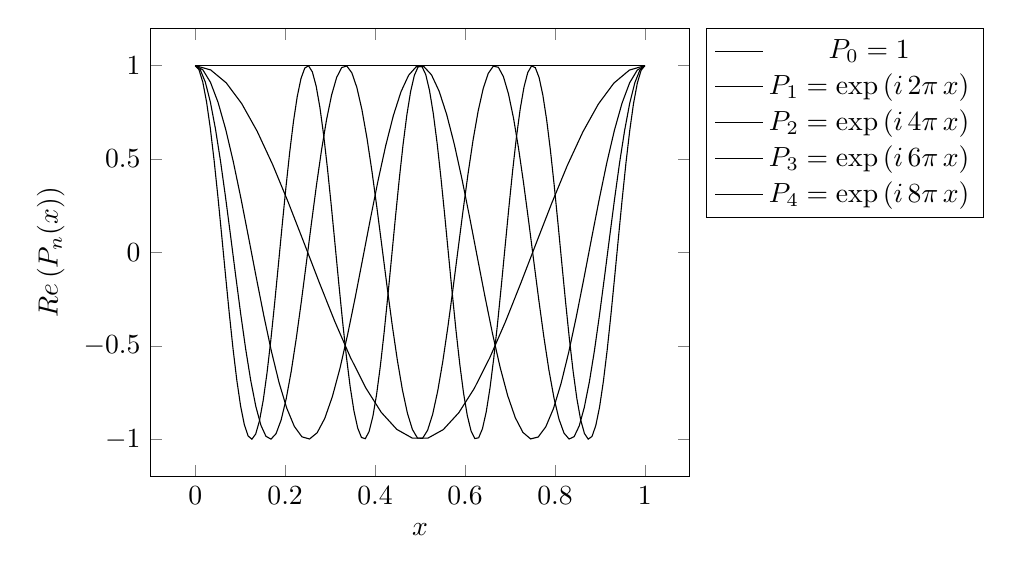
\begin{tikzpicture}
\begin{axis}[
  xlabel=$x$,
  ylabel=$\operatorname{Re}\left(P_n(x)\right)$,
  legend pos=outer north east]
\addplot[samples=2, domain=0:1] {1};
\addlegendentry{$P_0 = 1$};

\addplot[samples=30, domain=0:1] {cos(deg(6.28*x))};
\addlegendentry{$P_1 = \exp\left(i \, 2\pi \, x\right)$};

\addplot[samples=60, domain=0:1] {cos(deg(2*6.28*x))};
\addlegendentry{$P_2 = \exp\left(i \, 4\pi \, x\right)$};

\addplot[samples=90, domain=0:1] {cos(deg(3*6.28*x))};
\addlegendentry{$P_3 = \exp\left(i \, 6\pi \, x\right)$};

\addplot[samples=120, domain=0:1] {cos(deg(4*6.28*x))};
\addlegendentry{$P_4 = \exp\left(i \, 8\pi \, x\right)$};
\end{axis}
\end{tikzpicture}
\caption{The real parts of the first five basis functions of the Fourier expansion.}
\label{fig:fourier}
\end{figure}

Perform linear regression in modes.

% in practice


In our investigations, we will follow the argumentation of \textcite{melenk2001} and expand it to utilize \hp-coarsening as well.


We generate transformation matrices on the reference cell only. Simple matrix multiplication suffices in converting the solution from the finite element approximation into the series expansion.

Both strategies only on reference cell.


In practice, we will apply these considerations only on the reference cell in the finite element context. This way we only have to perform the costly calculation of transformation matrices for the determination of expansion coefficients just once and are able to reuse them later.

We can create one transformation. We can thus  by a simple matrix multiplication.

\begin{align}
L_{ij} = \frac{2i+1}{2} \int\limits_K P_i(x) \, \Psi_j \, \differential{x}
\end{align}
and
\begin{align}
a_i = L_{ij} u_j
\end{align}

On the downside, these transformations only yield applicable results if mapping from the reference to the actual cell is linear, resulting in a constant Jacobi determinant.

Further for practical calculations, we limit the number of basis functions used for all considerations up to these from which we think they have no contribution.

In practice, we noticed that this strategy offers poor results on linear elements. We suspect that linear polynomials do not offer sufficient information to make a well-founded statement about the smoothness attribute of the finite element approximation on the cell itself. We thus suggest to refrain from using them in this context and work with at least quadratic elements instead.

\cite{davydov2017} determine coefficients in every direction and perform least squares fit, and then take. We do not consider this approach in out investigations.

Sobolev regularity estimation. \textcite{ainsworth1998}. \textcite{houston2003}. \textcite[Sec.~2.4]{houston2005}

These strategies will be basis of future enhancements of decision strategies for \hp-adaptation.